\documentclass[a4paper, oneside]{discothesis}

\usepackage[utf8]{inputenc}
\usepackage[T1]{fontenc}

\usepackage{graphicx}
\usepackage{booktabs}
\usepackage{multirow}
\usepackage{amsmath}
\usepackage{subcaption}
\usepackage{xcolor}
\usepackage{siunitx}
\usepackage{algorithm}
\usepackage{algpseudocode}

%%%%%%%%%%%%%%%%%%%%%%%%%%%%%%%%%%%%%%%%%%%%%%%%%%%%%%%%%%%%%%%%%%%%%%%%%%%%%%%%%%%%%%%%%%%%%%%%%
% DOCUMENT METADATA

\thesistype{Semester Project} % Master's Thesis, Bachelor's Thesis, Semester Thesis, Group Project
\title{ML-based Deep Bitstream Inspection for
serverless FPGAs}

\author{Santiago de Heredia Tenorio}
\email{sdeheredia@ethz.ch}

\institute{Systems Group \\[2pt]
ETH Zürich}

% Optionally, you can put in your own logo here
% \logo{
\includegraphics[width=0.2\columnwidth]{figures/disco_logo_faded}}

\supervisors{Maximilian Heer\\[2pt] Prof.\ Dr.\ Gustavo Alonso}

% Optionally, keywords and categories of the work can be shown (on the Abstract page)
%\keywords{Keywords go here.}
%\categories{ACM categories go here.}

\date{\today}

%%%%%%%%%%%%%%%%%%%%%%%%%%%%%%%%%%%%%%%%%%%%%%%%%%%%%%%%%%%%%%%%%%%%%%%%%%%%%%%%%%%%%%%%%%%%%%%%%

\begin{document}

\frontmatter % do not remove this line
\maketitle

\cleardoublepage

\begin{acknowledgements}
	I thank Lorem ipsum dolor sit amet, consetetur sadipscing elitr, sed diam nonumy eirmod tempor invidunt ut labore et dolore magna aliquyam erat, sed diam voluptua. At vero eos et accusam et justo duo dolores et ea rebum. Stet clita kasd gubergren, no sea takimata sanctus est Lorem ipsum dolor sit amet. Lorem ipsum dolor sit amet, consetetur sadipscing elitr, sed diam nonumy eirmod tempor invidunt ut labore et dolore magna aliquyam erat, sed diam voluptua. At vero eos et accusam et justo duo dolores et ea rebum. Stet clita kasd gubergren, no sea takimata sanctus est Lorem ipsum dolor sit amet.
\end{acknowledgements}


\begin{abstract}
Cloud and serverless FPGA platforms expose reconfigurable fabric to user-supplied designs, making them vulnerable to malicious circuits such as ring oscillators. Prior work on ML-based bitstream inspection has shown that malicious payloads can be detected from bitstream-level patterns, but these approaches are generally evaluated as offline software classifiers and are not designed for low-latency deployment on datacenter-grade FPGA infrastructure. This motivates an online inspection approach in which the detection model itself is implemented in FPGA fabric and integrated into a cloud-oriented FPGA shell before user bitstreams are deployed.

This report investigates whether malicious-bitstream detection can be moved into the FPGA deployment path itself. We generate a dataset of benign Coyote partial bitstreams and trojan ring-oscillator bitstreams, represent bitstreams as image-like inputs, train compact CNN classifiers, and synthesize selected models using hls4ml. We evaluate the resulting design space across classification quality, input resolution, model depth, quantization, pruning, reuse factor, latency, and FPGA resource utilization.

Our results show that [main accuracy/F1/FNR result], while synthesized models achieve [latency] with [LUT/DSP/BRAM] utilization. We further integrate [selected model/downsampler] into the Coyote flow, demonstrating [end-to-end result]. The findings suggest that FPGA-resident ML-based inspection is feasible under [conditions], but remains limited by [main limitation].

\end{abstract}
\tableofcontents

\mainmatter % do not remove this line

% Start writing here
\chapter{Introduction}
\label{sec:introduction}

Field-programmable gate arrays (FPGAs) are increasingly used as datacenter accelerators because they provide programmable hardware with high performance and energy efficiency. In cloud and serverless settings, this programmability enables users to submit hardware applications that are deployed on shared FPGA infrastructure. Partial reconfiguration (PR) makes this model practical by allowing user logic to be loaded into a reconfigurable region while the trusted FPGA shell remains active.

This deployment model creates a security-critical boundary. The user-provided partial bitstream becomes an input to the platform, and loading it into the FPGA fabric may expose shared physical resources such as power delivery, thermal headroom, routing infrastructure, and neighboring workloads. Malicious circuits based on ring oscillators (ROs) are a representative threat: at scale, RO arrays can generate high-frequency switching activity, waste power, induce voltage drops, and cause denial-of-service or fault effects.

Existing cloud FPGA platforms show that bitstream validation is a practical concern. Prior attacks on AWS F1 demonstrated that malicious power-hammering designs could pass platform checks and crash instances. More recent work on AWS F2 suggests that HLS-generated power-wasting designs can still bypass deployment flows. These examples motivate inspection mechanisms that complement static platform checks and operate before partial reconfiguration.

Machine-learning-based bitstream inspection is a promising direction because prior work has shown that bitstream-derived representations contain learnable structure and can be used to classify malicious designs. However, most ML-based approaches are evaluated as offline software classifiers. This leaves a systems gap: a serverless FPGA platform needs a checker that fits the deployment path. Such a checker should be accurate enough to reject suspicious bitstreams, small enough to coexist with platform and user logic, and fast enough to avoid dominating PR latency.

This project studies whether ML-based malicious-bitstream inspection can move into the FPGA deployment path itself. Instead of relying on host-side CPU or GPU inspection, we explore a compact FPGA-resident checker for Coyote-style serverless FPGA systems. The checker receives a user partial bitstream, applies a deterministic byte-stream preprocessing step, runs a synthesized CNN classifier, and produces an accept/reject decision or suspiciousness score before PR.

We evaluate this idea using a dataset of benign Coyote application partial bitstreams and RO-based malicious partial bitstreams. Each bitstream is transformed into a fixed-size image-like tensor through deterministic resizing. We then train CNN classifiers, explore input resolution and model depth, synthesize selected candidates with hls4ml, and evaluate the resulting hardware designs across detection quality, false-positive and false-negative behavior, latency, and FPGA resource overhead.

This report makes four contributions:

\begin{enumerate}
    \item \textbf{Partial-bitstream dataset.}
    We construct a Coyote-oriented dataset from benign application partial bitstreams and RO-based malicious payloads.

    \item \textbf{Datacenter FPGA setting.}
    We evaluate inspection in a Coyote-style deployment setting with partial reconfiguration, multitenancy, and UltraScale+-class FPGA hardware.

    \item \textbf{ML-to-hardware inspection path.}
    We connect CNN training to hls4ml synthesis and evaluate whether trained bitstream classifiers can become practical FPGA-resident checkers.

    \item \textbf{Hardware-aware design-space evaluation.}
    We compare candidate models across detection quality, FNR/FPR, ROC AUC, LUT usage, BRAM usage, DSP usage, and added inspection latency.
\end{enumerate}

The main result is that FPGA-resident ML bitstream inspection is feasible as a deployment-path defense-in-depth mechanism. Among the synthesized candidates, the 256$\times$7 CNN provides the preferred deployment point because it balances useful detection quality with lower latency and substantially lower BRAM overhead than the larger 512$\times$7 alternative. Overall, the prototype shows a practical path from user-submitted partial bitstreams to a hardware-backed checker before deployment.

\chapter{Background, Threat Model, and Gap}
\label{ch:background-threat-gap}

\section{Serverless FPGAs and Partial Reconfiguration}
\label{sec:serverless-fpgas}

Serverless FPGA systems expose reconfigurable hardware as an on-demand acceleration service. Users submit hardware applications, while the platform manages the FPGA shell, host interface, memory system, networking, and runtime services~\cite{korolija2020os,ramhorst2025coyote,mainas2025f3}. This model hides low-level FPGA management from users and allows the provider to share FPGA capacity across applications.

Partial reconfiguration makes this deployment model practical. The FPGA is divided into a static region and one or more reconfigurable regions. The static region contains trusted platform logic, while the reconfigurable region contains user logic. A user application can therefore be loaded without rebuilding the full FPGA image.

This structure creates a natural security boundary. The user partial bitstream enters the platform before it is loaded into the reconfigurable region. If the bitstream contains malicious logic, the platform may configure that logic directly into shared FPGA fabric. The deployment path should therefore include an inspection step before partial reconfiguration.

Coyote is a relevant target for this work because it provides a datacenter FPGA shell with partial reconfiguration, multitenancy, and platform services~\cite{korolija2020os,ramhorst2025coyote}. It gives a concrete setting for studying whether bitstream inspection can become part of the FPGA deployment path.

\section{Ring-Oscillator Payloads}
\label{sec:ring-oscillators}

Ring oscillators are a simple and well-studied malicious payload for FPGAs~\cite{gnad2017voltage,la2020fpgadefender,la2021denial,provelengios2020power}. A ring oscillator is built from an odd feedback loop of inverters. The loop has no stable state and continuously toggles. A single ring oscillator is small, but a large array of attacker-controlled ring oscillators can create high-frequency switching activity.

This switching activity stresses shared physical resources. In a cloud or serverless FPGA setting, the relevant resources include power delivery, thermal headroom, and neighboring user logic. Large ring-oscillator arrays can waste power, induce voltage drops, cause denial of service, or trigger timing faults. For this reason, RO-based payloads are a useful first target for malicious-bitstream inspection.

This work focuses on detecting RO-based malicious partial bitstreams. This is a narrow threat class, but it is realistic enough to test the core systems question. The main goal is to evaluate whether a learned detector can be accurate, small, and fast enough to sit in the deployment path.

\section{Threat Model}
\label{sec:threat-model}

We consider a serverless FPGA platform with a trusted shell and an untrusted user partial bitstream. The attacker can submit a syntactically valid partial bitstream for the user reconfigurable region. The bitstream may contain an RO-based payload designed to stress shared physical resources after configuration.

The attacker's goal is to have the malicious bitstream accepted and loaded through partial reconfiguration. The platform's goal is to inspect the bitstream before configuration and reject suspicious inputs.

The checker is placed before the partial reconfiguration step. It receives the incoming partial bitstream, preprocesses it into the fixed input format expected by the classifier, and outputs a decision.

\section{Prior Work}
\label{sec:prior-work}

FPGA security surveys provide the broader context for bitstream-level attacks and defenses~\cite{jin2020security,zhang2019recent}. For this report, the most relevant defenses fall into three groups. Cloud and vendor checks are practical because they are integrated into deployment flows, but they usually target known rule violations~\cite{giechaskiel2019measuring,la2021denial}. Structural methods search for suspicious circuit patterns, such as self-oscillators, but can depend strongly on device architecture and bitstream structure~\cite{la2020fpgadefender,provelengios2020power,yoon2018bret}. ML-based methods learn patterns from bitstream-derived data, but are commonly evaluated as offline software classifiers~\cite{rettkowski2019inspection,chaudhuri2022detection,elnaggar2023learning,palumbo2022trojan,stahlesmith2025realtime}.

\begin{table}[t]
    \centering
    \caption{Comparison of approaches for malicious FPGA bitstream detection.}
    \label{tab:prior-work-gap}

    \small
    \setlength{\tabcolsep}{5pt}
    \renewcommand{\arraystretch}{1.18}

    \begin{tabularx}{\linewidth}{
        @{}
        >{\hsize=0.80\hsize}Y
        >{\hsize=1.05\hsize}Y
        >{\hsize=1.15\hsize}Y
        >{\hsize=1.00\hsize}Y
        @{}
    }
        \toprule
        \textbf{Approach} &
        \textbf{Strength} &
        \textbf{Limitation} &
        \textbf{Relation to this work} \\
        \midrule

        Cloud and vendor checks &
        Already integrated into deployment flows &
        Restricted to known rules and platform policies &
        Complemented by learned inspection \\
        \addlinespace[0.45em]

        Structural RO analysis &
        Detects oscillator structures directly &
        Often architecture-specific and difficult to generalize &
        Avoids explicit structural reverse engineering \\
        \addlinespace[0.45em]

        ML-based inspection &
        Learns patterns directly from bitstream data &
        Commonly evaluated as an offline software classifier &
        Moves the learned detector into FPGA fabric \\
        \midrule

        \textbf{This work} &
        Connects partial-bitstream classification with hardware synthesis &
        Evaluates one platform and one primary threat class &
        Studies detection quality, hardware cost, and deployment-path integration \\
        \bottomrule
    \end{tabularx}
\end{table}
Prior ML-based work is important because it shows that bitstream-derived representations contain learnable structure~\cite{rettkowski2019inspection,chaudhuri2022detection,elnaggar2023learning,palumbo2022trojan}. CNNs and other classifiers can distinguish benign and malicious bitstreams without fully decoding the circuit semantics. Recent work by Stahle-Smith and Karakchi is especially close in motivation because it uses static byte-level features for malicious-bitstream detection and deploys the selected classifier on a PYNQ-Z1 embedded platform~\cite{stahlesmith2025realtime}. That work uses byte-frequency features, TSVD, SMOTE, and a Random Forest for embedded-system detection. This report instead studies deterministic byte-image tensors, CNN classifiers, hls4ml synthesis, and integration into a Coyote-style U55C deployment path. The remaining question is whether such inspection can satisfy the constraints of a serverless FPGA deployment path.

\section{Research Gap}
\label{sec:research-gap}


The gap addressed in this report is deployment-oriented ML inspection. Offline classification alone is not enough for a serverless FPGA platform. A useful checker must satisfy three requirements.

\begin{table}[H]
    \centering
    \caption{Feasibility dimensions for FPGA-resident bitstream inspection.}
    \label{tab:feasibility-dimensions}
    \begin{tabular}{p{0.22\linewidth} p{0.43\linewidth} p{0.25\linewidth}}
        \toprule
        \textbf{Dimension} & \textbf{Question} & \textbf{Metrics} \\
        \midrule
        Detection quality &
        Does the checker retain useful security coverage? &
        F1, FNR, FPR, ROC AUC \\
        \midrule
        Hardware cost &
        Can the checker fit beside platform and user logic? &
        Latency, LUT, BRAM, DSP \\
        \midrule
        Integration &
        Can the checker sit on the Coyote partial-reconfiguration path? &
        PR-path placement and prototype design \\
        \bottomrule
    \end{tabular}
\end{table}



This report studies all three dimensions together. We generate Coyote-style partial bitstreams, train CNN classifiers on deterministic byte-image representations, synthesize selected models with hls4ml, and evaluate whether the resulting hardware designs are practical candidates for deployment-path inspection.


\chapter{Dataset and Preprocessing}
\label{ch:dataset-preprocessing}

\section{Dataset Goal}
\label{sec:dataset-goal}

The goal of the dataset is to evaluate malicious-bitstream inspection on the same type of artifact that appears in a serverless FPGA deployment path. The input to the checker is a partial bitstream, not source code, a netlist, or an implementation report. The dataset is therefore built from Coyote-style partial bitstreams.

The classification task is binary. Benign samples are partial bitstreams generated from Coyote applications. Malicious samples are partial bitstreams that contain ring-oscillator payloads. Labels are assigned by construction from the generation flow.

This dataset is designed to test deployment-like variation. Samples are generated across different floorplans and configurations so that the classifier is not evaluated on a single fixed placement. The malicious class also includes higher-density RO samples to evaluate how detection changes as the RO footprint increases.

\section{Bitstream Generation}
\label{sec:bitstream-generation}

Benign samples are generated from real Coyote applications. These applications represent normal user accelerators that could be deployed into a reconfigurable region. To increase variation, the applications are built across multiple floorplans and configurations.

The benign catalog contains eight debug-enabled Coyote applications: hello world, HLS vector add, multitenancy AES, user interrupts, perf FPGA, multithreading AES, Euclidean distance, and cosine similarity. It also contains no-debug variants for seven of these applications. In the available manifests, this gives 120 debug-enabled benign samples and 101 no-debug benign samples.

Malicious samples are generated from RO-based designs. These designs place attacker-controlled ring oscillators into the reconfigurable region. The RO count is varied to create payloads with different logic footprints. This allows the evaluation to distinguish between small low-footprint payloads and larger high-density payloads.

Figure~\ref{fig:dataset-pipeline} shows the dataset generation flow. Both benign and malicious designs pass through the same floorplan and configuration sweep before partial-bitstream generation. The output is a labeled dataset of partial bitstreams and metadata.

\begin{figure}[t]
    \centering
    % Figure generated locally from figures/dataset_generation_pipeline.dot.
    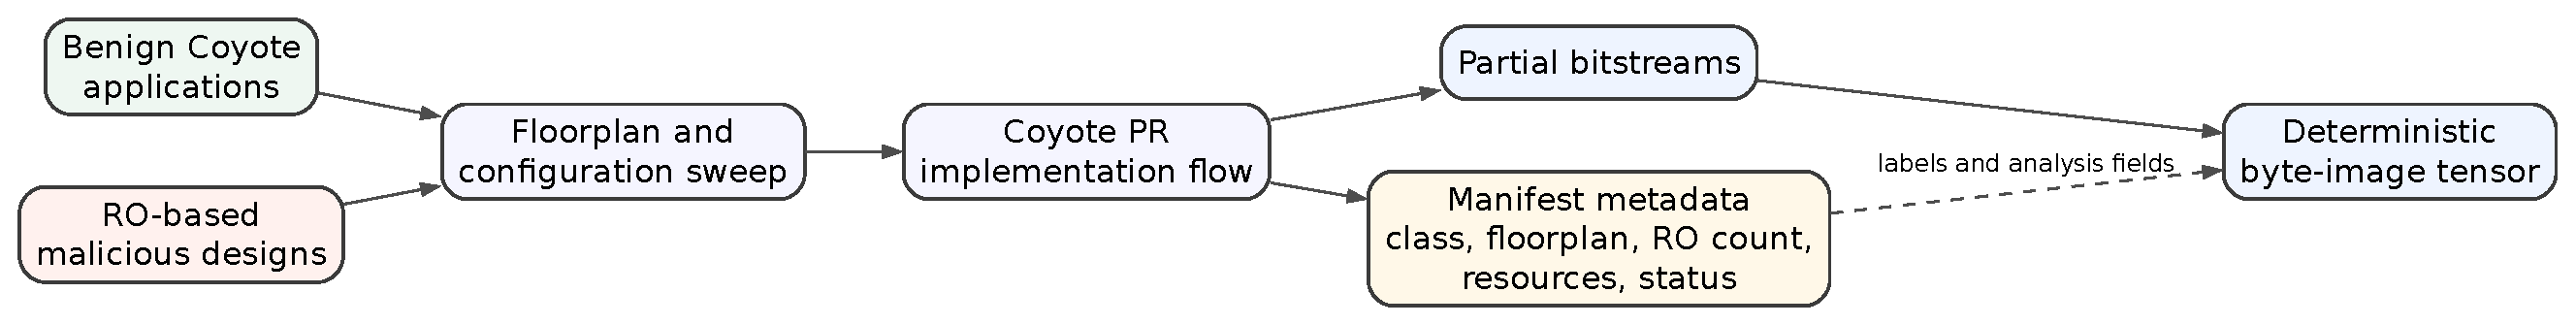
\includegraphics[width=0.95\linewidth]{figures/dataset_generation_pipeline.pdf}
    \caption{Dataset generation pipeline. Benign Coyote applications and RO-based malicious designs are generated across deployment-like variation and converted into labeled partial bitstreams.}
    \label{fig:dataset-pipeline}
\end{figure}

\section{Dataset Composition}
\label{sec:dataset-composition}

Table~\ref{tab:dataset-composition} summarizes the available generated dataset. The original generated corpus contains benign Coyote bitstreams and normal-RO malicious bitstreams across 15 floorplans, FP00--FP14. The higher-density big-RO extension uses six of those floorplans and is kept separate because it is used for the extended footprint evaluation.

The available generated manifests contain 221 benign samples, 225 normal-RO malicious samples, and 78 big-RO malicious samples. The normal-RO corpus spans 33 RO-count settings. The big-RO extension spans 13 higher-density RO-count settings.

\begin{table}[t]
    \centering
    \caption{Dataset composition by class and RO category.}
    \label{tab:dataset-composition}
    \small
    \resizebox{\linewidth}{!}{
    \begin{tabular}{@{}l l l r r@{}}
        \toprule
        \textbf{Class} & \textbf{Source} & \textbf{Variation} & \textbf{Floorplans} & \textbf{Samples} \\
        \midrule
        % Sources: ../ml_deep_bitstream_inspection/datasets/full_dataset_it{1,2,3}/artifacts/manifest_available.csv
        Benign &
        Coyote applications &
        8 apps, 7 no-debug variants &
        15 &
        221 \\
        \midrule
        % Sources: ../ml_deep_bitstream_inspection/datasets/full_dataset_it{1,2,3}/artifacts/manifest_available.csv
        Normal RO &
        Standalone RO payloads &
        33 RO-count settings &
        15 &
        225 \\
        \midrule
        % Source: ../ml_deep_bitstream_inspection/datasets/full_dataset_it4_big_ro/artifacts/manifest_available.csv
        Big RO &
        Higher-density RO payloads &
        13 RO-count settings &
        6 &
        78 \\
        \bottomrule
    \end{tabular}
    }
\end{table}

Each sample also stores metadata used during analysis. This includes the design source, floorplan, configuration, label, bitstream size, and estimated RO footprint when applicable. The RO footprint metadata is used later to evaluate whether misses concentrate in small malicious designs.

\section{Preprocessing}
\label{sec:preprocessing}

The preprocessing step converts each partial bitstream into the fixed input shape expected by the CNN. The transform is intentionally simple. It does not reverse-engineer the bitstream. It does not extract hand-crafted circuit features. It treats the partial bitstream as a byte stream.

Each bitstream is read as a sequence of bytes
\[
    b = [b_0, b_1, \ldots, b_n].
\]
The sequence is resized to a fixed number of bytes. If the bitstream is longer than the target size, it is downsampled. If it is shorter, it is padded. The result is reshaped into a grayscale image-like tensor.

The main input resolutions are
\[
    128^2,\quad 256^2,\quad 512^2.
\]
Larger resolutions are also used during model exploration to measure how much classification quality improves when more bitstream detail is preserved.

This representation is useful for two reasons. First, it gives CNNs a fixed-size input while preserving byte-level structure from across the bitstream. Second, the operation is simple enough to implement in FPGA logic before inference. This matters because the final goal is an FPGA-resident checker that can run in the deployment path.

\section{Dataset Limitations}
\label{sec:dataset-limitations}

The dataset supports a feasibility study. It does not cover every malicious FPGA design. The malicious class focuses on RO-based payloads, and labels are assigned by construction. This means the classifier may learn artifacts that correlate with maliciousness, such as payload size, routing density, or floorplan effects.

The extended RO-footprint evaluation helps address this issue by showing where the detector is strong and where it is weak. Small RO payloads remain the harder case. Larger RO payloads are more relevant for power-stress attacks and are evaluated separately in Section~\ref{ch:cnn-pipeline}.


\chapter{CNN Inspection Pipeline}
\label{ch:cnn-pipeline}

\section{Choice of CNNs}
\label{sec:cnn-choice}

We use convolutional neural networks because prior work has shown that bitstream-derived representations contain learnable structure. Rettkowski et al. studied neural-network-based inspection of partial FPGA bitstreams. Chaudhuri and Chakrabarty used CNN-based learning to detect malicious FPGA bitstreams. Elnaggar et al. also used CNNs as part of a malicious-circuit detection pipeline. These results support the idea that bitstreams can be treated as structured data for classification, even without full bitstream reverse engineering~\cite{rettkowski2019partialbitstreams,chaudhuri2022cnnbitstreams,elnaggar2023learning}.

This project follows the same direction, but with a different systems goal. The model is not only trained for software accuracy. It must also be small enough and regular enough to synthesize into FPGA logic. CNNs are a good fit for this because they can operate on fixed-size image-like tensors and can be converted to hardware using tools such as hls4ml.

The classifier receives the preprocessed bitstream tensor from Chapter~\ref{ch:dataset-preprocessing}. The output is a binary prediction. The positive class is the RO-based malicious class. The negative class is the benign Coyote application class.

\section{Model Input and Classification Task}
\label{sec:model-input-task}

Each partial bitstream is converted into a grayscale image-like tensor through deterministic resizing. The tensor does not represent a natural image. It is a fixed-size layout of byte values sampled from the bitstream. This gives the CNN local neighborhoods of byte values from which it can learn statistical and spatial patterns.

The main classification task is binary:
\[
    y =
    \begin{cases}
        0, & \text{benign Coyote partial bitstream},\\
        1, & \text{RO-based malicious partial bitstream}.
    \end{cases}
\]

The main metrics are accuracy, F1, true positive rate, false positive rate, false negative rate, and ROC AUC. False negatives are especially important because they correspond to malicious bitstreams that would be accepted by the checker.

\section{Design Space}
\label{sec:cnn-design-space}

The CNN design space is explored in stages. The goal is to preserve useful detection quality while keeping the final hardware design practical. We therefore vary the model only along dimensions that affect both classification and hardware cost.

\begin{table}[t]
    \centering
    \caption{CNN design-space dimensions.}
    \label{tab:cnn-design-space}
    \begin{tabular}{p{0.24\linewidth} p{0.38\linewidth} p{0.26\linewidth}}
        \toprule
        \textbf{Dimension} & \textbf{Question} & \textbf{Main metrics} \\
        \midrule
        Input resolution &
        How much bitstream detail is retained &
        F1, FNR, ROC AUC \\
        \midrule
        CNN depth &
        How much model capacity is needed &
        F1, TPR, FPR \\
        \midrule
        Quantization &
        How little precision is enough &
        AUC, hls4ml parity, resources \\
        \midrule
        Pruning &
        How much sparsity can be introduced &
        AUC, sparsity, synthesis impact \\
        \bottomrule
    \end{tabular}
\end{table}

The main software sweep varies input resolution and depth. The tested resolutions include smaller inputs such as $128^2$ and larger inputs such as $256^2$ and $512^2$. Higher resolutions preserve more bitstream detail, but they also increase the cost of the synthesized checker. The depth sweep evaluates whether additional convolutional layers improve detection enough to justify the hardware cost.

\section{Software Detection Results}
\label{sec:software-detection-results}

Figure~\ref{fig:f1-resolution-depth} shows the main software result. F1 improves as input resolution and model depth increase. Small inputs lose information during resizing. Larger inputs preserve more byte-level structure and give the CNN more useful signal. Deeper models also improve classification up to the evaluated range.

\begin{figure}[t]
    \centering
    % Replace with the exported F1 heatmap from the presentation.
    % Recommended file name: figures/f1_resolution_depth.pdf
    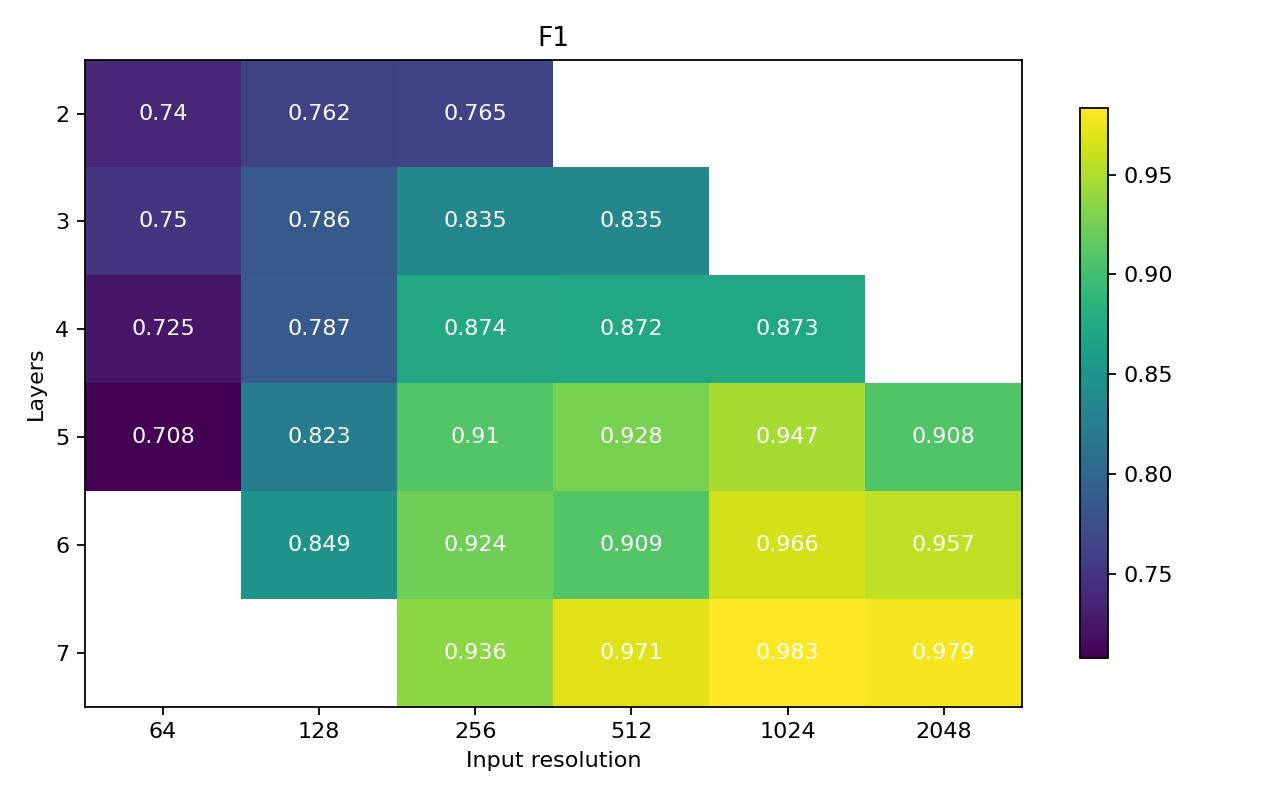
\includegraphics[width=0.82\linewidth]{figures/f1_resolution_depth.pdf}
    \caption{F1 score across input resolution and CNN depth. Higher resolution and deeper models improve software detection quality, but they also increase hardware cost.}
    \label{fig:f1-resolution-depth}
\end{figure}

The strongest software models are not automatically the best deployment candidates. Larger inputs improve F1, but they also increase memory pressure, latency, and resource usage after synthesis. The later hardware evaluation therefore focuses on deployable candidates rather than only the maximum-F1 software model.

\begin{table}[t]
    \centering
    \caption{Representative software CNN results.}
    \label{tab:software-cnn-results}
    \begin{tabular}{l r r r r}
        \toprule
        \textbf{Model} & \textbf{Resolution} & \textbf{Depth} & \textbf{F1} & \textbf{Role} \\
        \midrule
        256$\times$7 & $256^2$ & 7 & TODO & Deployment candidate \\
        512$\times$7 & $512^2$ & 7 & TODO & Accuracy-oriented candidate \\
        1024$\times$7 & $1024^2$ & 7 & TODO & Software upper-bound candidate \\
        \bottomrule
    \end{tabular}
\end{table}

\section{Interpretability Check}
\label{sec-interpretability}

We use Grad-CAM as a qualitative sanity check. The goal is to inspect whether the CNN focuses on localized regions of the bitstream image or behaves as if it only learned a trivial global statistic.

\begin{figure}[t]
    \centering
    % Optional. Replace with the Grad-CAM figure from the presentation.
    % Recommended file name: figures/gradcam_example.pdf
    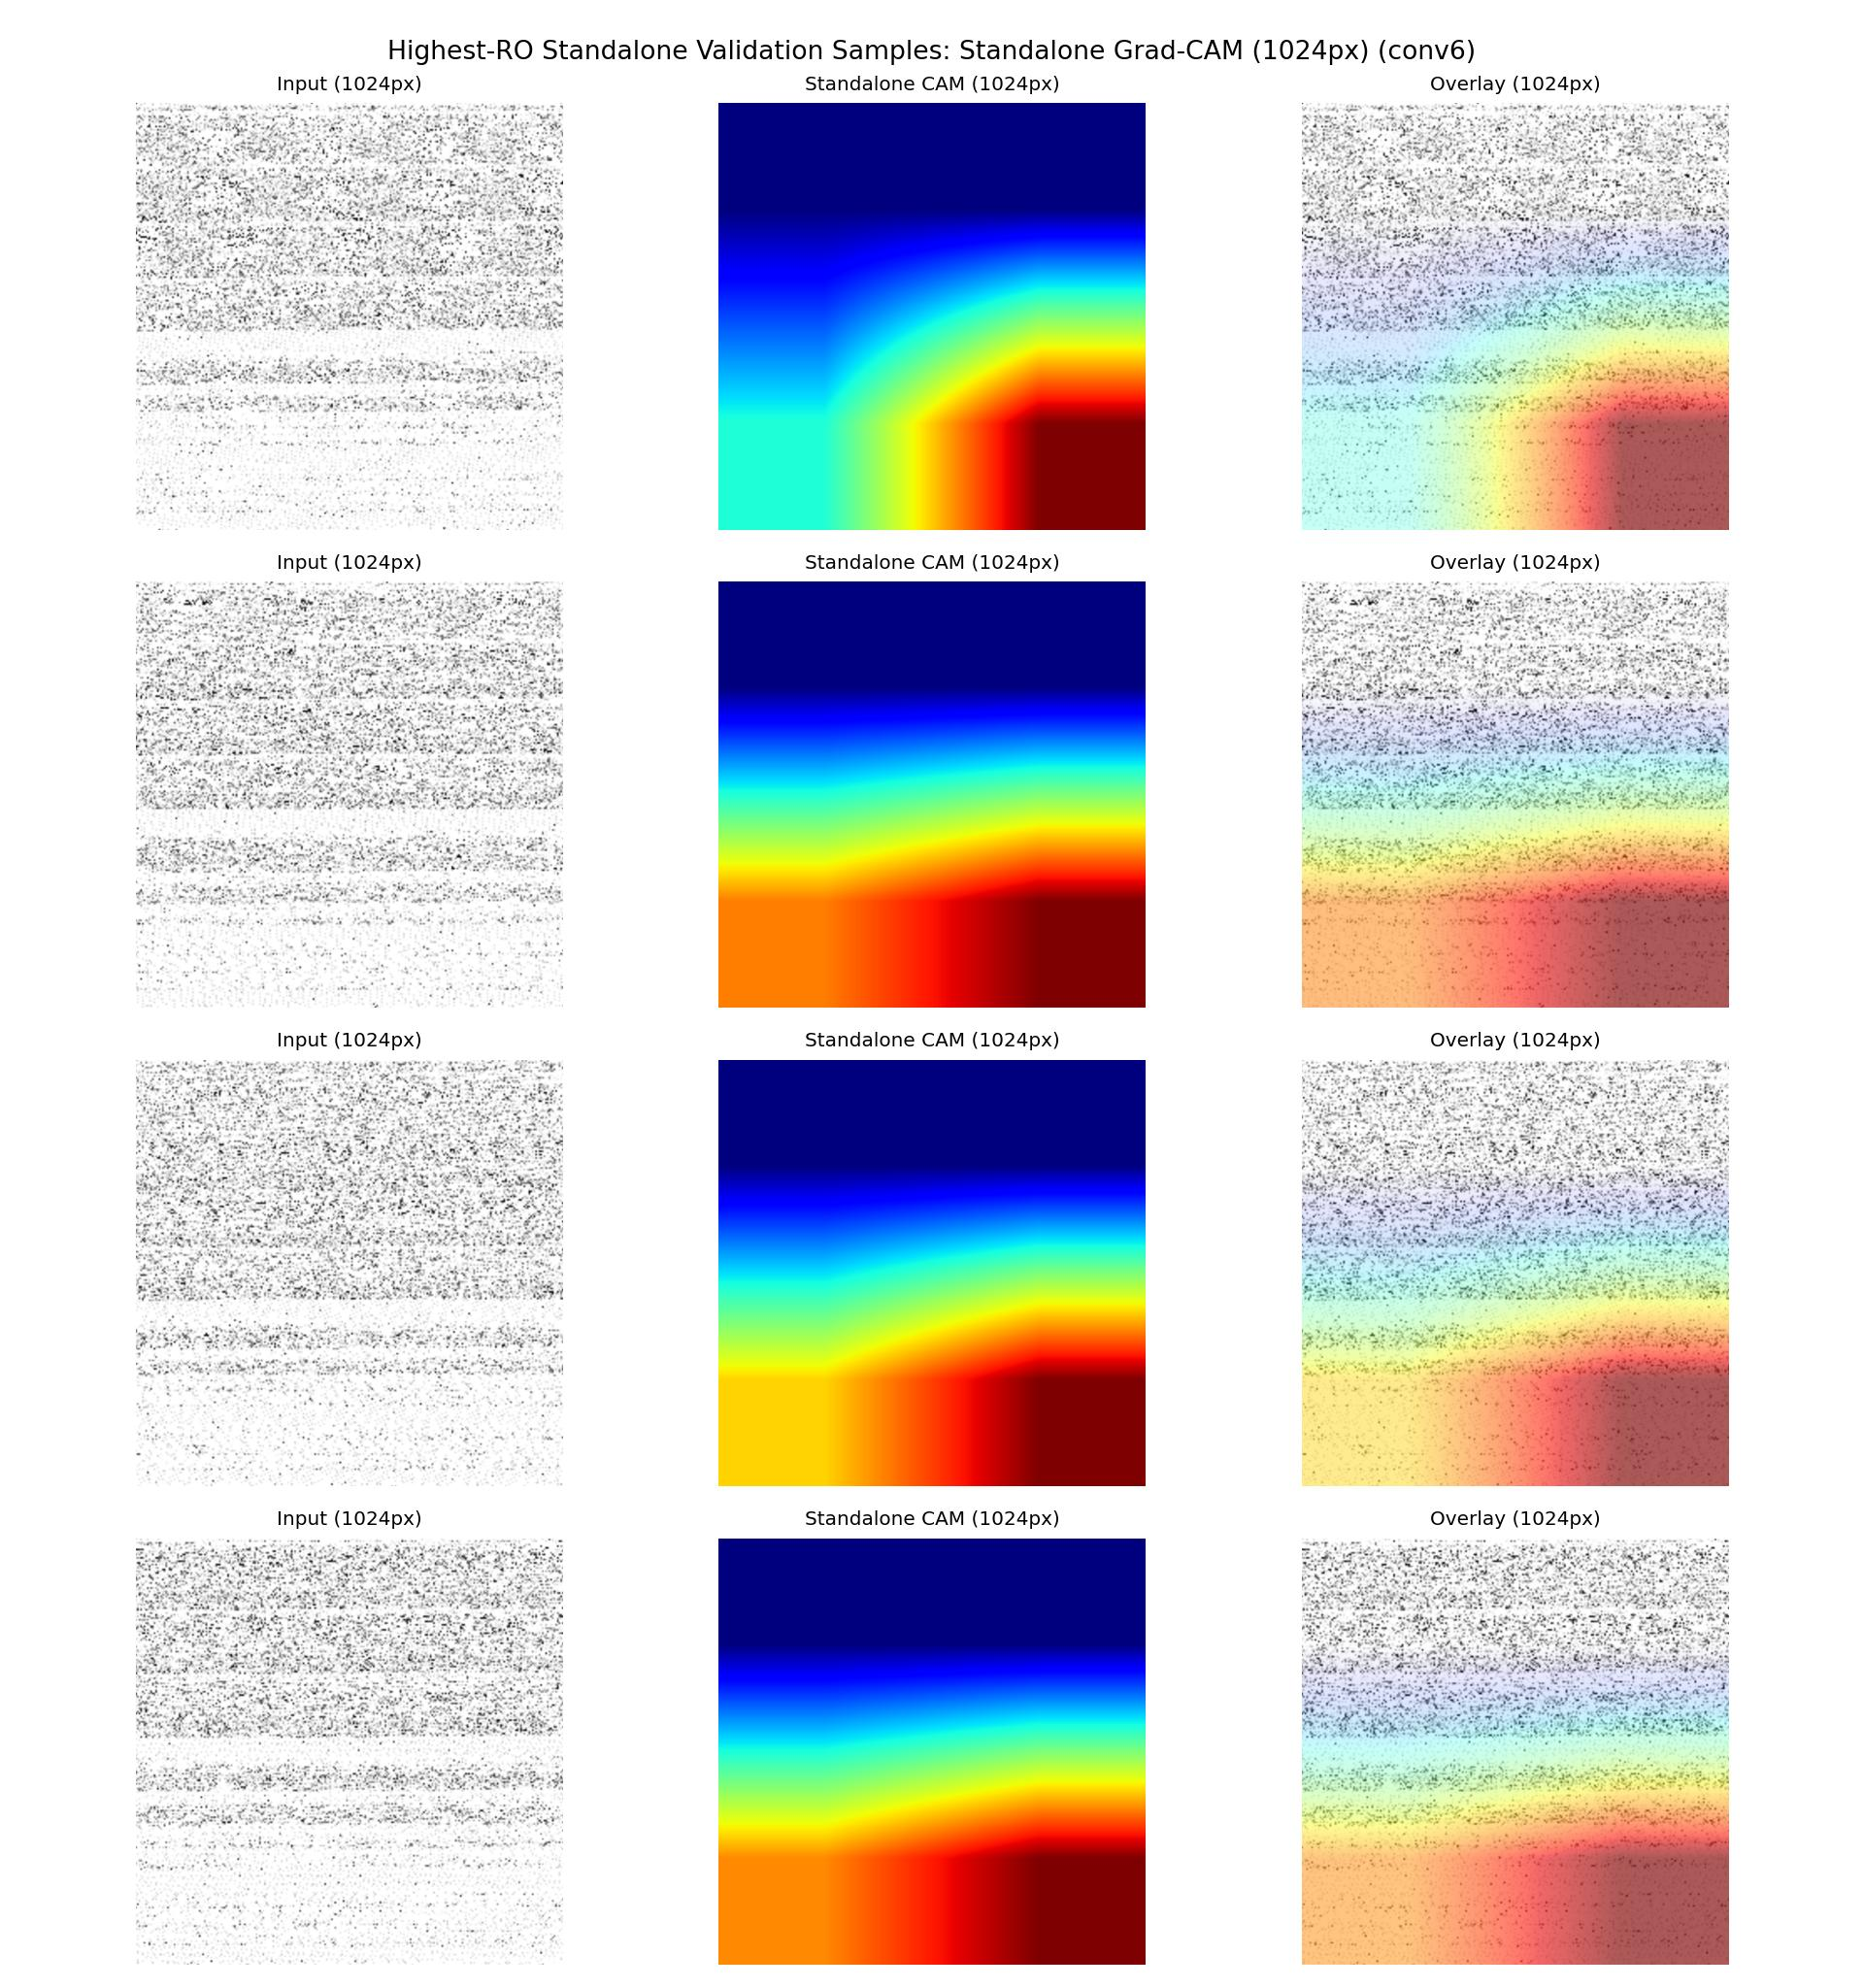
\includegraphics[width=0.82\linewidth]{figures/gradcam_example.pdf}
    \caption{Grad-CAM example for a malicious prediction. The highlighted regions show which parts of the bitstream image contribute most to the classifier output.}
    \label{fig:gradcam-example}
\end{figure}

The Grad-CAM examples show localized regions and bands with higher contribution. This supports the use of a spatial bitstream representation. It does not prove that the model identifies ring oscillators at the circuit level. It is only a qualitative check on the learned representation.

\section{Extended RO-Footprint Evaluation}
\label{sec:ro-footprint-evaluation}

The original dataset tests whether the classifier can separate benign Coyote bitstreams from RO-based malicious bitstreams. We also evaluate how detection changes as the RO footprint increases. This matters because high-density RO payloads are more relevant for power-stress and timing-fault scenarios.

Figure~\ref{fig:ro-footprint-detection} shows the extended RO-footprint result. Misses concentrate in the smallest RO-footprint bin. Detection becomes reliable for larger evaluated payloads. This suggests that the classifier is strongest for high-density RO attacks, while low-footprint payloads remain the harder case.

\begin{figure}[t]
    \centering
    % Replace with the exported RO-footprint plot from the presentation.
    % Recommended file name: figures/ro_footprint_detection.pdf
    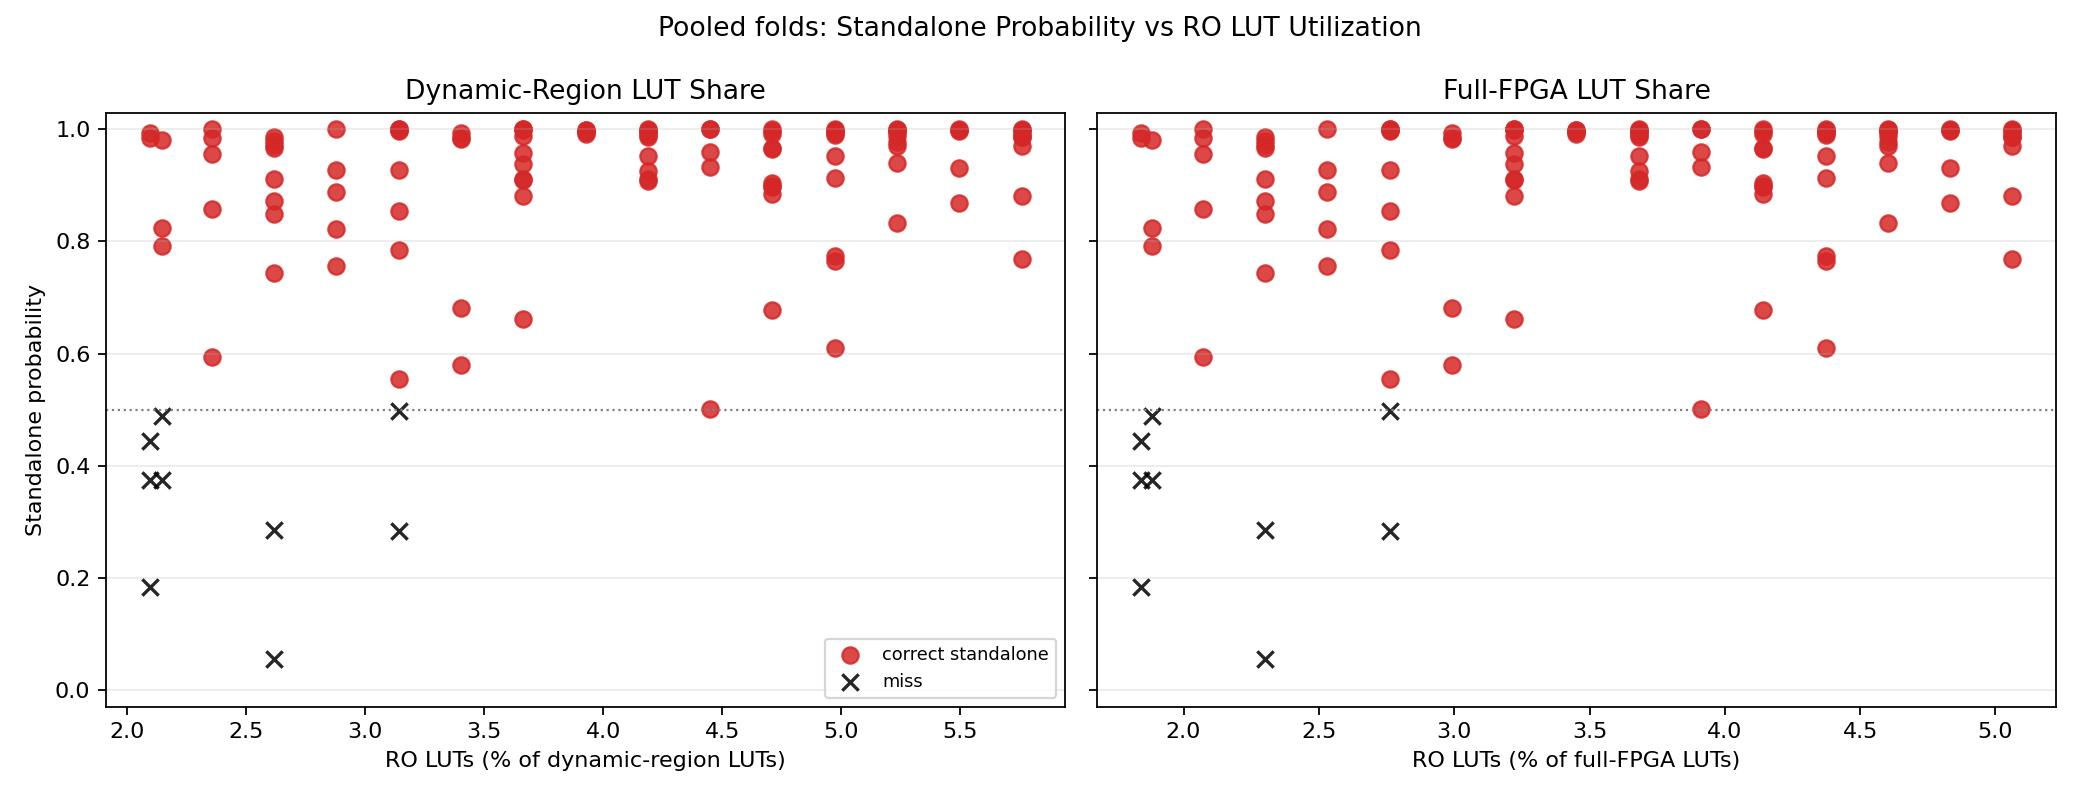
\includegraphics[width=0.82\linewidth]{figures/ro_footprint_detection.pdf}
    \caption{Detection across RO-footprint bins. Smaller RO payloads are harder to detect, while larger evaluated payloads are detected more reliably.}
    \label{fig:ro-footprint-detection}
\end{figure}

This result is important for interpreting the detector. The model does not provide complete coverage against all malicious circuits. It provides useful coverage for RO-based payloads, especially larger payloads that are more likely to create practical power-stress effects. The next chapter evaluates whether these CNN candidates can be synthesized into practical FPGA-resident checkers.

\chapter{hls4ml Synthesis and Hardware Results}
\label{ch:hls4ml-results}

\section{Synthesis Goal}
\label{sec:synthesis-goal}

The CNN models from Chapter~\ref{ch:cnn-pipeline} are useful only if they can be mapped to practical FPGA hardware. The goal of this chapter is to evaluate whether the trained classifiers can become deployment-path checkers with acceptable latency and resource overhead.

We use hls4ml to convert trained CNN models into hardware designs~\cite{duarte2018fast,aarrestad2021fast}. The synthesis flow takes a trained Keras or QKeras model~\cite{coelho2020qkeras}, generates an HLS implementation, validates the generated design with C simulation, and produces latency and resource estimates after synthesis. The final W8A8 candidates are trained with QKeras quantization-aware training before hls4ml conversion, so the software model already uses the quantized weight and activation behavior evaluated by the hardware flow. The final candidates are then evaluated in terms of added latency and added FPGA resources relative to the Coyote baseline.

The main hardware metrics are LUT usage, BRAM usage, DSP usage, and added inspection latency. The main detection metrics are accuracy, F1, true positive rate, false positive rate, and ROC AUC. The final design point should balance both groups of metrics.

\section{hls4ml Flow}
\label{sec:hls4ml-flow}

The hardware flow starts from a trained CNN. The model is exported and passed to hls4ml. hls4ml generates C++ code and an HLS project. We then run C simulation to check that the generated model produces outputs consistent with the software model. After this parity check, the design is synthesized and evaluated.

The flow is:

\begin{center}
\small
\begin{tabular}{c}
\textbf{trained CNN} $\rightarrow$ \textbf{hls4ml conversion} $\rightarrow$ \textbf{C simulation} \\[3pt]
$\rightarrow$ \textbf{HLS synthesis} $\rightarrow$ \textbf{latency and resource report}
\end{tabular}
\end{center}

This flow is repeated for selected CNN candidates. We do not synthesize every software model. Larger software models can improve F1, but they can also produce hardware designs that are too slow or too resource-heavy. The synthesis stage therefore acts as a filter between high-quality software models and deployable FPGA checkers.

\section{Hardware Tuning Parameters}
\label{sec:hls4ml-knobs}

The main hls4ml tuning parameters are quantization, reuse factor, synthesis strategy, and manual per-layer configuration.

Quantization controls the precision of weights and activations. Lower precision can reduce hardware cost, but it can also reduce model quality or create numerical differences between the software model and the generated HLS model.

The reuse factor controls how much hardware is shared across operations. A low reuse factor increases parallelism and reduces latency. It also increases resource usage. A high reuse factor uses fewer resources but increases latency.

The synthesis strategy controls whether hls4ml optimizes more aggressively for latency or resource usage. We also use manual per-layer tuning because a single global setting is often too coarse. Some layers dominate latency, while others dominate BRAM or DSP usage.

Table~\ref{tab:hls4ml-knobs} summarizes the main knobs.

\begin{table}[t]
    \centering
    \caption{hls4ml tuning parameters used during synthesis.}
    \label{tab:hls4ml-knobs}
    \begin{tabular}{p{0.25\linewidth} p{0.45\linewidth} p{0.20\linewidth}}
        \toprule
        \textbf{Parameter} & \textbf{Effect} & \textbf{Main tradeoff} \\
        \midrule
        Quantization &
        Sets weight and activation precision &
        Quality vs. area \\
        \midrule
        Reuse factor &
        Controls hardware sharing across operations &
        Latency vs. area \\
        \midrule
        Strategy &
        Selects resource-oriented or latency-oriented mapping &
        Area vs. speed \\
        \midrule
        Per-layer tuning &
        Adjusts important layers individually &
        Practical fit \\
        \bottomrule
    \end{tabular}
\end{table}

\section{Latency and Resource Tradeoff}
\label{sec:hls4ml-tradeoff}

The HLS exploration shows a clear tradeoff between detection quality, latency, and resource usage. Larger input resolutions preserve more bitstream detail and improve software F1. They also increase the cost of the hardware checker. Lower reuse factors reduce latency but require more parallel hardware. Higher reuse factors reduce hardware use but increase latency.

Figure~\ref{fig:hls-tradeoff} shows the W8A8 P50 resource-strategy sweep. Circles and squares show reuse-factor sweeps for the 256$\times$7 and 512$\times$7 models. The starred points show the manually tuned v1 candidates used for deployment evaluation. These manual candidates keep the same reported F1 as the corresponding resource-strategy sweep while reducing latency and LUT utilization.

\begin{figure}[t]
    \centering
    % Source image copied from ../ml_deep_bitstream_inspection/hls4ml/results/selected_feasible_candidates_resource_strategy/plots/latency_lut_f1_tradeoff.png
    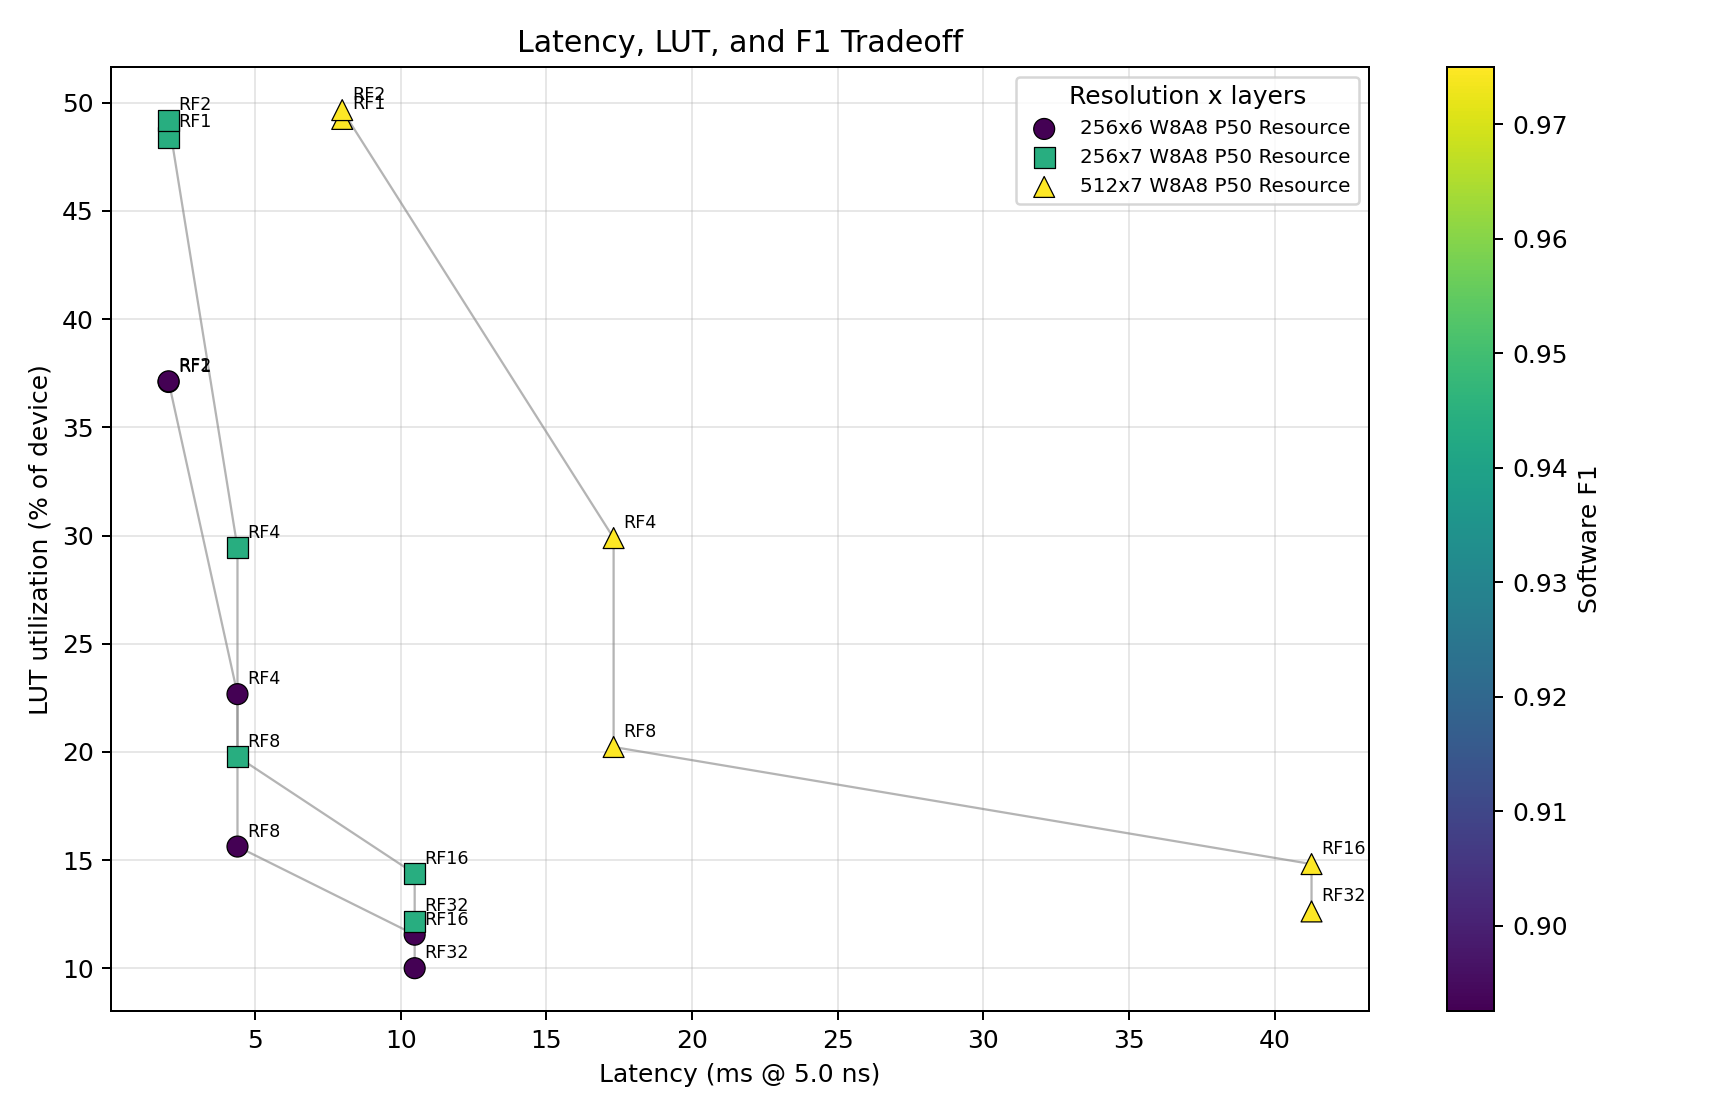
\includegraphics[width=0.92\linewidth]{figures/hls_latency_resource_f1_resource_strategy.png}
    \caption{Latency, LUT utilization, and F1 tradeoff for W8A8 P50 resource-strategy candidates. Marker shapes distinguish the 256$\times$7 and 512$\times$7 reuse-factor sweeps from the manually tuned v1 deployment candidates.}
    \label{fig:hls-tradeoff}
\end{figure}

Figure~\ref{fig:hls-latency-f1-frontier} and  Figure~\ref{fig:hls-lut-f1-frontier} show the broader design-space frontier. Unless the design is hand-optimized per CNN layer, better F1 generally requires a larger latency budget. The same pattern appears for LUT utilization. Higher-quality models are available, but they move rightward on the latency and LUT axes. The hand-optimized points are important because they shift selected candidates toward the useful frontier instead of accepting the default global resource-strategy mapping.

\begin{figure}[t]
    \centering
    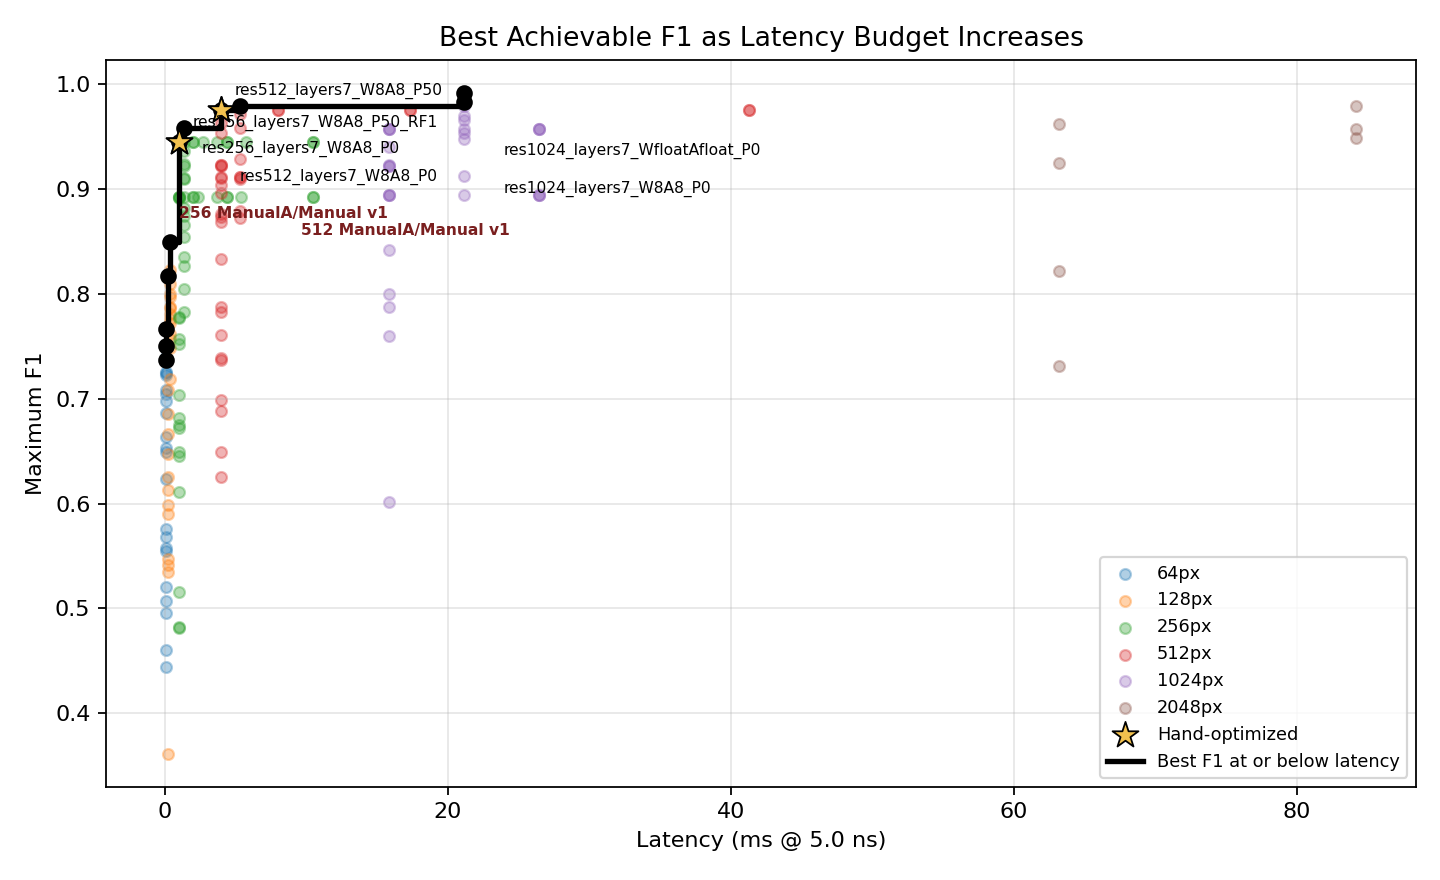
\includegraphics[
        width=\linewidth,
        trim={0 5mm 0 3mm},
        clip
    ]{figures/hls_latency_f1_frontier.png}

    \caption{
        Best achievable F1 as the latency budget increases.
        The black frontier shows the maximum F1 achieved by any synthesized
        candidate within each latency budget. Stars indicate the manually
        optimized deployment candidates.
    }
    \label{fig:hls-latency-f1-frontier}
\end{figure}

\begin{figure}[t]
    \centering
    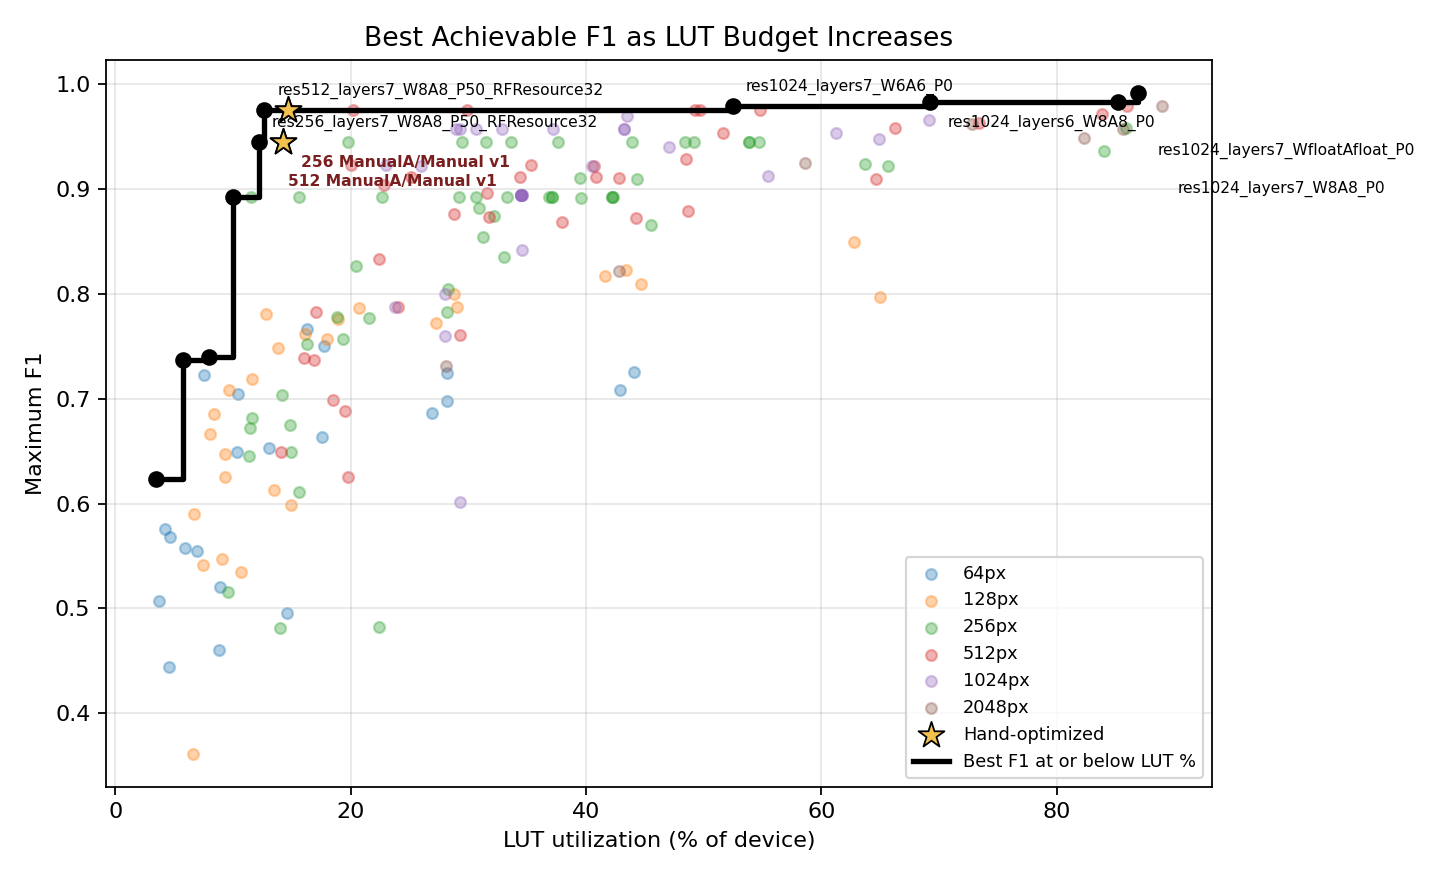
\includegraphics[
        width=\linewidth,
        trim={0 5mm 0 3mm},
        clip
    ]{figures/hls_lut_f1_frontier.png}

    \caption{
        Best achievable F1 as the LUT budget increases.
        The black frontier shows the maximum F1 achieved by any synthesized
        candidate within each LUT budget. Stars indicate the manually
        optimized deployment candidates.
    }
    \label{fig:hls-lut-f1-frontier}
\end{figure}

\section{Final Synthesized Candidates}
\label{sec:final-synthesized-candidates}

The final comparison focuses on two synthesized models. The 256$\times$7 model is the preferred deployment candidate. The 512$\times$7 model is the accuracy-oriented alternative. 

Table~\ref{tab:final-candidates} shows the final comparison. Classification metrics are evaluated on the original small-RO test set unless stated otherwise. The extended TPR is measured on the extended RO-footprint dataset.

\begin{table}[t]
    \centering
    \caption{Final synthesized candidates. Resource percentages are routed hls4ml wrapper/user-logic attribution on the target U55C.}
    \label{tab:final-candidates}
    \resizebox{\linewidth}{!}{
    \begin{tabular}{l r r r r r r r r r r}
        \toprule
        \textbf{Model} &
        \textbf{Acc.} &
        \textbf{F1} &
        \textbf{TPR} &
        \textbf{TPR Ex.} &
        \textbf{FPR} &
        \textbf{AUC} &
        \textbf{Latency} &
        \textbf{LUT} &
        \textbf{BRAM} &
        \textbf{DSP} \\
        \midrule
        % Source: ../ml_deep_bitstream_inspection/hls4ml/reproducibility/prod_res256_coyote_accel_downsampler_hls4ml_e2e_20260524/results/performance_summary.json
        256$\times$7 &
        87.7\% &
        88.5\% &
        92.0\% &
        98.7\% &
        16.9\% &
        95.1\% &
        3.35 ms &
        +4.47\% &
        +17.86\% &
        +14.72\% \\
        \midrule
        % Source: ../ml_deep_bitstream_inspection/hls4ml/reproducibility/prod_res512_coyote_accel_downsampler_hls4ml_e2e_20260524/results/performance_summary.json
        512$\times$7 &
        90.4\% &
        90.5\% &
        89.3\% &
        100.0\% &
        8.45\% &
        96.9\% &
        6.53 ms &
        +4.90\% &
        +61.78\% &
        +14.45\% \\
        \bottomrule
    \end{tabular}
    }
\end{table}

The 512$\times$7 model has higher accuracy, higher F1, lower false positive rate, higher ROC AUC, and perfect TPR on the extended RO-footprint dataset. This makes it the stronger detection candidate.

The 256$\times$7 model is the better deployment candidate. It has lower added latency and much lower BRAM overhead. Its F1 is only two percentage points lower than the 512$\times$7 model, and its original-set TPR is higher. The BRAM difference is the main reason for preferring 256$\times$7. The routed hierarchy attributes 61.78\% of device BRAM to the 512$\times$7 checker wrapper, while the 256$\times$7 wrapper accounts for 17.86\%.

\section{Latency Context}
\label{sec:latency-context}

The added inspection latency should be interpreted relative to the latency of partial reconfiguration and serverless invocation. Table~\ref{tab:latency-context} compares the 256$\times$7 and 512$\times$7 inspection latencies with F3 and generic serverless reference points~\cite{mainas2025f3,ustiugov2021stellar}.

\begin{table}[t]
    \centering
    \caption{Added inspection latency relative to deployment and serverless latency references.}
    \label{tab:latency-context}
    \begin{tabular}{p{0.46\linewidth} r r r}
        \toprule
        \textbf{Context} & \textbf{Baseline} & \textbf{256$\times$7} & \textbf{512$\times$7} \\
        \midrule
        F3 warm path with reconfiguration &
        141 ms &
        +2.38\% &
        +4.63\% \\
        \midrule
        Coyote PR on VU9P with 6\% PR region &
        6.04 ms &
        +55.46\% &
        +108.11\% \\
        \midrule
        Coyote PR on VU9P with 33\% PR region &
        36.94 ms &
        +9.07\% &
        +17.68\% \\
        \midrule
        Coyote PR on VU9P with 66\% PR region &
        73.27 ms &
        +4.57\% &
        +8.91\% \\
        \midrule
        Generic FaaS cold invocation median &
        448 ms &
        +0.75\% &
        +1.46\% \\
        \bottomrule
    \end{tabular}
\end{table}

The added latency is small relative to full serverless invocation latencies and larger PR operations. It is more significant for very small PR regions. This suggests that FPGA-resident inspection is most attractive when the checker is used in realistic deployment paths where PR and runtime overheads already dominate a few milliseconds of inference time.

The 256$\times$7 model adds 3.35 ms. The 512$\times$7 model adds 6.53 ms. Both are plausible for deployment-path inspection, but the smaller model gives a safer latency budget.

\section{Resource Context}
\label{sec:resource-context}

The baseline Coyote design uses 10.26\% of LUTs and 9.77\% of BRAM on the target device. It uses no URAM or DSPs in the reported baseline. The checker adds resources on top of this baseline.

Table~\ref{tab:resource-context} summarizes the baseline and the added checker overhead.

\begin{table}[t]
    \centering
    \caption{Baseline Coyote resource usage and routed checker wrapper/user-logic attribution.}
    \label{tab:resource-context}
    \begin{tabular}{l r r r r}
        \toprule
        \textbf{Design} & \textbf{LUT} & \textbf{BRAM} & \textbf{URAM} & \textbf{DSP} \\
        \midrule
        Baseline Coyote &
        10.26\% &
        9.77\% &
        0\% &
        0\% \\
        \midrule
        % Source: ../ml_deep_bitstream_inspection/hls4ml/reproducibility/prod_res256_coyote_accel_downsampler_hls4ml_e2e_20260524/results/performance_summary.json
        Added 256$\times$7 checker &
        +4.47\% &
        +17.86\% &
        +1.15\% &
        +14.72\% \\
        \midrule
        % Source: ../ml_deep_bitstream_inspection/hls4ml/reproducibility/prod_res512_coyote_accel_downsampler_hls4ml_e2e_20260524/results/performance_summary.json
        Added 512$\times$7 checker &
        +4.90\% &
        +61.78\% &
        +1.77\% &
        +14.45\% \\
        \bottomrule
    \end{tabular}
\end{table}

The LUT overhead is similar for both synthesized candidates. DSP overhead is also similar. BRAM is the limiting resource. This makes the 256$\times$7 candidate more attractive for integration because it leaves more memory resources available for the shell, services, and user logic.

\section{Quantization and Pruning}
\label{sec:quantization-pruning-results}

Quantization and pruning are evaluated as hardware-aware compression techniques~\cite{coelho2020qkeras,han2016deepcompression}. Quantization reduces arithmetic precision. Pruning removes weights and increases sparsity. Both can reduce the cost of a neural network, but the benefit depends on the synthesis flow and on whether the generated hardware can exploit the reduced precision or sparsity. For the selected W8A8 models, quantization is not applied only after training. We use QKeras quantization-aware training so the model learns under the target 8-bit weight and activation quantizers.

For quantized models, we check both software quality and hls4ml parity. This is important because a low-bit model can have good software accuracy but still produce mismatches after conversion. For pruned models, we track actual sparsity and classification quality. Sparse models are useful only if sparsity translates into lower synthesis cost or better feasibility.

In the final design selection, quantization and pruning are treated as supporting tools. The main deployment decision is driven by the synthesized 256$\times$7 and 512$\times$7 candidates, where measured latency and resource overhead are available.

\section{Takeaway}
\label{sec:hls4ml-takeaway}

The hardware results show that FPGA-resident CNN inspection is feasible, but the design point matters. The 512$\times$7 model gives stronger detection metrics, especially lower FPR, higher ROC AUC, and perfect TPR on the extended RO-footprint dataset. It also has much higher BRAM overhead and roughly double the latency of the 256$\times$7 model.

The 256$\times$7 model is the preferred candidate for further Coyote integration. It provides useful detection quality, lower added latency, and much lower BRAM overhead. It is the better balance between security coverage and deployment cost.


\chapter{Proposed Coyote Integration}
\label{ch:coyote-integration}

\section{Integration Point}
\label{sec:coyote-integration-point}

The final goal is to place the bitstream checker directly on the Coyote deployment path. In this path, a user bitstream reaches the platform before partial reconfiguration. The checker should inspect the bitstream before it is loaded into the reconfigurable region.

Coyote provides a suitable target because it already separates platform services from user logic~\cite{korolija2020os,ramhorst2025coyote}. The static shell manages host communication, memory services, networking, command handling, and runtime control. User accelerators are deployed into reconfigurable regions. This structure gives a clear location for inspection before the partial reconfiguration step.

Figure~\ref{fig:coyote-integration} shows the proposed placement. The checker receives the user partial bitstream, applies preprocessing, runs the synthesized CNN, and returns a decision to the deployment logic.

\begin{figure}[t]
    \centering
    % Figure generated locally from figures/coyote_integration_path.dot.
    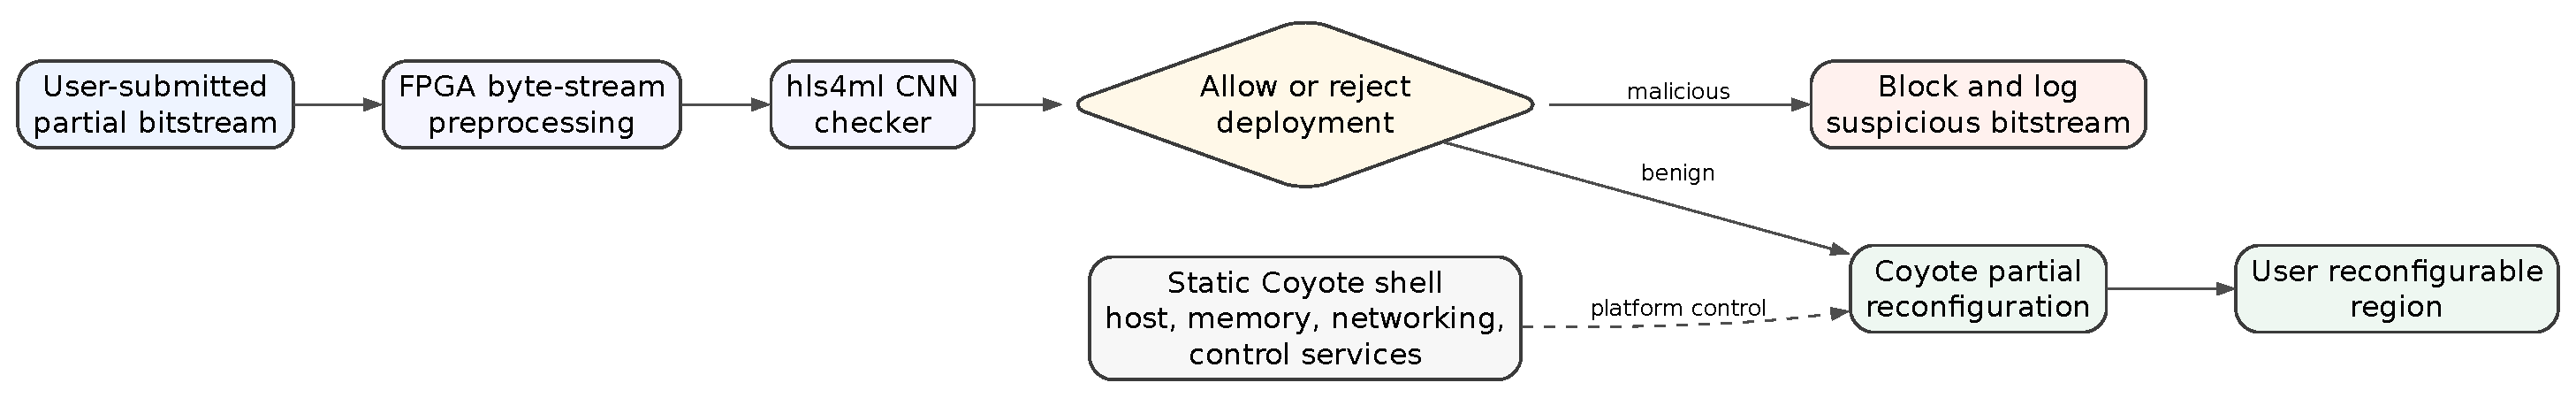
\includegraphics[width=0.95\linewidth]{figures/coyote_integration_path.pdf}
    \caption{Proposed Coyote integration path. The partial-bitstream checker is placed before partial reconfiguration and decides whether the bitstream should be loaded or rejected.}
    \label{fig:coyote-integration}
\end{figure}

\section{Checker Flow}
\label{sec:checker-flow}

The checker follows the same pipeline used during model evaluation. The incoming partial bitstream is treated as a byte stream. The preprocessing logic resizes the stream into the fixed tensor shape expected by the CNN. The synthesized hls4ml model then produces a maliciousness score or binary prediction.

The deployment logic uses this output to control partial reconfiguration. If the score is below the rejection threshold, the bitstream is allowed to continue to the PR controller. If the score is above the threshold, the platform blocks the reconfiguration and logs the event.

The intended flow is:

\begin{center}
\small
\begin{tabular}{c}
\textbf{user bitstream} $\rightarrow$ \textbf{preprocessing} $\rightarrow$ \textbf{CNN checker} \\[3pt]
$\rightarrow$ \textbf{allow or reject} $\rightarrow$ \textbf{partial reconfiguration}
\end{tabular}
\end{center}

This design keeps inspection inside the FPGA deployment path. It avoids a separate host-side inspection stage and gives the platform a self-contained gate before loading user logic. This follows the broader goal of making FPGA-resident ML components deployable inside systems paths rather than treating them only as offline models~\cite{heer2025ml4sys}.

\section{Prototype Scope}
\label{sec:coyote-prototype-scope}

This work evaluates the main components needed for such an integration. The preprocessing method has already been implemented as HLS C++ raw-byte downsampling logic, lowered to Verilog by the HLS flow, and used for the deployment-oriented latency results. The CNN candidates are synthesized with hls4ml and evaluated for latency and resource cost.

The current integration is still a proposal and prototype direction. A complete Coyote deployment would require control-plane integration, threshold policy, logging, error handling, and validation with the real PR controller. It would also need a clear policy for low-confidence predictions.


\chapter{Discussion, Limitations, and Future Work}
\label{ch:discussion}

\section{Discussion}
\label{sec:discussion}

The results show that FPGA-resident ML inspection is a feasible direction for serverless FPGA deployment. The checker can be placed before partial reconfiguration, trained CNNs can classify Coyote-style partial bitstreams with useful accuracy, and hls4ml can synthesize selected models into concrete hardware candidates.

The main design lesson is that the best software model is not always the best deployment model. The 512$\times$7 candidate improves several detection metrics, including F1, false positive rate, ROC AUC, and extended RO-footprint detection. It also has much higher BRAM overhead and higher latency. The 256$\times$7 candidate gives a better deployment balance. It has lower added latency, much lower BRAM use, and still provides useful detection quality.

The checker should be understood as a defense-in-depth component. It can reduce the chance that an RO-based malicious bitstream reaches the reconfigurable region. It does not prove that a bitstream is safe. A practical platform should combine this checker with static validation, bitstream authentication, runtime monitoring, and platform policy~\cite{jin2020security,zhang2019recent,ahmed2022multitenant}.

The RO-footprint results also show where the detector is strongest. Larger RO payloads are detected more reliably. These payloads are the most relevant for power-stress attacks. Smaller payloads remain harder and require stronger datasets, better models, or additional checks.

\section{Limitations}
\label{sec:limitations}

This work is a feasibility study. It makes progress toward FPGA-resident inspection, but it has several limitations.

\begin{table}[t]
    \centering
    \caption{Current limitations of the prototype.}
    \label{tab:limitations}
    \begin{tabular}{p{0.28\linewidth} p{0.62\linewidth}}
        \toprule
        \textbf{Limitation} & \textbf{Impact} \\
        \midrule
        Binary classification &
        The current task distinguishes benign Coyote bitstreams from RO-based malicious bitstreams. It does not cover broader malicious-circuit classes. \\
        \midrule
        RO-focused dataset &
        The malicious class is generated from ring-oscillator payloads. Other attacks may produce different bitstream patterns. \\
        \midrule
        CNN-only evaluation &
        The main detector family is CNN-based. Other hardware-friendly classifiers may provide better latency or resource tradeoffs. \\
        \midrule
        Low-footprint attacks &
        Small malicious payloads are harder to detect. Misses concentrate in the smallest RO-footprint regime. \\
        \midrule
        One platform setting &
        The evaluation focuses on Coyote-style artifacts and one FPGA platform family. Generalization across devices and shells is not yet shown. \\
        \midrule
        Partial integration &
        The checker is synthesized and placed in a proposed Coyote path, but it is not yet a complete production deployment component. \\
        \bottomrule
    \end{tabular}
\end{table}

\section{Future Work}
\label{sec:future-work}

The next step is broader validation. The dataset should include more attack classes, more benign applications, and harder malicious examples. Important additions include timing attacks, side-channel circuits, covert channels, non-RO power wasters, and mixed benign-plus-malicious designs.

Low-footprint attacks need special attention. A stronger benchmark should include subtle payloads with varied RO densities and placements. This would test whether the classifier can detect malicious structure without relying on large payload size.

Future work should also evaluate other model families. MLPs, decision trees, tiny CNNs, binary neural networks, and FINN-style quantized models may provide better latency and resource tradeoffs~\cite{blott2018finnr,coelho2020qkeras,han2016deepcompression}. Netlist-oriented GNN classifiers are another possible direction for broader malicious-circuit coverage~\cite{alrahis2024malignnoma}. These models should be compared under the same dataset, metrics, and synthesis flow.

Generalization is another open question. The current results should be repeated across different FPGA families, floorplans, shells, and benign workloads. Versal or V80-class devices would be especially useful targets because they are relevant to newer datacenter FPGA deployments.

The final systems step is full Coyote integration. The checker should be connected directly to the PR control path, with threshold policy, logging, error handling, and a clear response for low-confidence predictions. This would turn the current prototype into a complete in-path security gate.


\chapter{Conclusion}
\label{ch:conclusion}

This project studied whether ML-based malicious-bitstream inspection can move into the FPGA deployment path for serverless FPGA systems. The target setting is a Coyote-style environment where user partial bitstreams are checked before partial reconfiguration. The goal is to add a hardware-backed security gate that can reject suspicious bitstreams before they enter the reconfigurable region.

We built a partial-bitstream inspection pipeline around three components. First, we generated a dataset with benign Coyote application bitstreams and RO-based malicious bitstreams. Second, we transformed each bitstream into a fixed-size byte-image tensor and trained CNN classifiers for binary detection. Third, we synthesized selected CNNs with hls4ml and evaluated their detection quality, latency, and FPGA resource overhead.

The results show that FPGA-resident ML inspection is feasible as a defense-in-depth mechanism. The 512$\times$7 W8A8 P50 manual-v1 model gives stronger accuracy-oriented metrics, including higher F1, lower false positive rate, higher ROC AUC, and perfect detection on the extended RO-footprint dataset. The 256$\times$7 W8A8 P50 manual-v1 model is the preferred deployment candidate because it gives a better hardware tradeoff. It achieves useful detection quality with 3.35 ms added latency and much lower BRAM overhead than the 512$\times$7 alternative.

The main takeaway is that deployment-oriented bitstream inspection must be evaluated across both ML and systems metrics. Software accuracy alone is not enough. A practical checker must also fit beside the FPGA shell and user logic, add limited latency to the PR path, and integrate cleanly into the deployment flow. This prototype shows a practical path toward such a checker, while leaving broader attack coverage, harder datasets, cross-platform validation, and full Coyote integration as future work.

\include{rest.tex}

% This displays the bibliography for all cited external documents. All references have to be defined in the file references.bib and can then be cited from within this document.
\bibliographystyle{IEEEtran}
\bibliography{references}

\appendix
\chapter{First Appendix Chapter Title}



\end{document}